\documentclass[12pt,onecolumn,draftclsnofoot]{IEEEtran}
\usepackage[a4paper,margin=1in]{geometry}
\usepackage{times,graphicx,amsmath,booktabs,cite,url}
\usepackage[ruled,linesnumbered]{algorithm2e}
\usepackage[table]{xcolor}
\usepackage{tikz,pgfplots,array}
\usetikzlibrary{arrows.meta,positioning,calc,fit}
\pgfplotsset{compat=1.16}

\begin{document}

\title{CodeWarden: Retrieval-Augmented Local LLM Pull Request Review with Layered Guardrails, Evaluated Against Rule-Based Baselines}

\author{Group 01: Agrima Agarwal (230639), Aaradhya Gupta (230644), Naveen Singh/Kiran Khatter\\
School of Engineering \& Technology, BML Munjal University}
\maketitle

\begin{abstract}
Code review is slow, and good reviewers need knowledge of the whole repository, yet most automated reviewers see only the changed lines and many send private code to hosted models. We present CodeWarden, a pull-request reviewer that runs a local code model, retrieves related repository code before it reviews a change, and wraps the model in layered guardrails for secrets, personal data, prompt injection and unsafe output. Existing work on automated review mostly measures the text similarity of generated comments; it rarely tests whether a reviewer finds known bugs, or whether repository context helps. We built a labelled benchmark of 19 files with 16 planted bugs in two suites, one with bugs visible in the diff and one with bugs that depend on repository conventions. We compared a regular-expression baseline, a local 7.6-billion-parameter model that reads only the diff, and the same model with retrieval. Every configuration ran three times, and we report mean and standard deviation. The local model found 83.3\% of the diff-visible bugs against 60.0\% for the baseline. On context-dependent bugs, retrieval raised recall from 50.0\% to 72.2\%, and four further retrieval settings stayed between 72.2\% and 77.8\%. Precision did not improve consistently, two bugs were never found, and the confidence intervals overlap, so the evidence is suggestive rather than conclusive. The code, benchmark and raw results are provided in the project repository.
\end{abstract}

\begin{IEEEkeywords}
code review, guardrails, large language models, pull requests, retrieval-augmented generation
\end{IEEEkeywords}

\noindent\textbf{Overleaf Project Link:} \url{https://www.overleaf.com/project/6afdca7574f49166a7984460}

\noindent\textbf{Git Repository:} \url{https://github.com/Agrima6/codewarden}

\section{Introduction}
Code review is one of the most widely used quality practices in software engineering. Studies of review at Microsoft and at Google show that developers use it to find defects, but also to share knowledge and to keep a codebase consistent~\cite{bacchelli2013expectations,sadowski2018modern}. At the same time, language models trained on source code can now read and write programs~\cite{chen2021codex,roziere2023codellama}, and open models of a few billion parameters, such as Qwen2.5-Coder~\cite{hui2024qwen}, run on a single laptop. This makes it realistic to give every pull request a first automated review without sending private code to an outside service, which matters to students, small teams and companies with confidentiality rules.

The difficulty is that a review comment is only useful when it is correct, and many bugs cannot be seen in the changed lines alone. A new request handler that forgets to check that the user is logged in, or that calls a helper function with the wrong argument type, is wrong only because of conventions and signatures defined elsewhere in the repository. A reviewer that reads just the diff cannot know this. Further risks come from the model itself: its output changes from run to run~\cite{ouyang2023nondeterminism}, AI assistants can produce insecure code~\cite{pearce2022asleep,perry2023insecure}, and text inside a pull request or a retrieved file can carry instructions aimed at the model rather than at the human reader~\cite{greshake2023indirect,perez2022ignore}. A practical reviewer must therefore be both accurate and safe to run on untrusted input.

Research on automated review has trained or prompted models for tasks such as comment generation and code refinement~\cite{tufano2021towards,li2022codereviewer,lu2023llamareviewer,guo2023chatgpt,tang2024codeagent}. These studies are valuable, but the tasks they score differ from the question a developer asks of a reviewer: given a change that contains a bug, does the tool point to the right line, and how often does it raise a false alarm? Retrieval of repository context is known to help code completion~\cite{zhang2023repocoder,ding2023crosscodeeval}. To our knowledge, the studies we surveyed do not test, with a no-retrieval control and repeated runs, whether the same idea helps a small local model find planted bugs in pull requests. Because language-model output is non-deterministic, a single run of any such comparison can also mislead.

We therefore ask two research questions.
\begin{itemize}
 \item \textbf{RQ1:} Does a local language-model reviewer find more known bugs than a rule-based baseline?
 \item \textbf{RQ2:} Does retrieving related repository code improve the recall of the local reviewer on bugs that depend on repository context, and what happens to its precision?
\end{itemize}

To answer them we built CodeWarden, an open pull-request reviewer, and a small labelled benchmark. This paper makes four contributions.
\begin{itemize}
 \item A reviewer architecture that combines a local model, retrieval over the repository, and fifteen guardrails on input, model output, published text and GitHub actions.
 \item A benchmark of 19 files with 16 planted bugs in two suites: one where the bug is visible in the diff, and one where it depends on repository conventions.
 \item A controlled evaluation of a rule-based baseline, the model without retrieval and the model with retrieval, each run three times, with confidence intervals computed per distinct bug.
 \item An ablation over the number of retrieved chunks and the retrieval method, and a failure analysis that reports results which did not replicate.
\end{itemize}
We study a deliberately small and fully controlled setting. RQ1 checks that the model is worth its cost against something simple and free, and RQ2 checks the specific idea that repository context is what closes the gap. Every number in the paper comes from files saved by our own evaluation scripts, and where an early result did not replicate we say so instead of choosing the better run.
The rest of the paper is organised as follows. Section~\ref{sec:related} reviews related work, Section~\ref{sec:background} gives the background and the formal problem, Section~\ref{sec:method} describes the method, Section~\ref{sec:setup} the experimental setup, Section~\ref{sec:results} the results, Section~\ref{sec:discussion} the discussion, and Section~\ref{sec:conclusion} concludes.


\section{Related Work}\label{sec:related}
We group the literature into five themes and then state the gap that this paper addresses.

\subsection{Code Review in Practice}
Bacchelli and Bird examined why developers review code and which challenges they face~\cite{bacchelli2013expectations}, and Sadowski et al. described how review works at Google~\cite{sadowski2018modern}. Both treat review as a human activity in which understanding the surrounding code is part of the job, and neither is about automation. They are the reason we judge a reviewer by whether a human could act on its comments: a comment must point to a real changed line and say what is wrong. This motivates giving an automated reviewer access to that surrounding code instead of only the diff.

\subsection{Learning-Based Review Automation}
Tufano et al. trained two deep-learning models, one that revises code before review and one that implements a reviewer's comment, and reported success in up to 16\% and 31\% of cases~\cite{tufano2021towards}. CodeReviewer pre-trains a model with four review-specific tasks on data from nine languages and outperforms earlier pre-trained approaches on quality estimation, comment generation and refinement~\cite{li2022codereviewer}. LLaMA-Reviewer fine-tunes LLaMA with fewer than 1\% trainable parameters and matches review-specific models~\cite{lu2023llamareviewer}. Prompting a general model also works: ChatGPT reached an exact-match score of 22.78 on code refinement against 15.50 for CodeReviewer~\cite{guo2023chatgpt}. CodeAgent uses several cooperating agents and a supervising checker for tasks that include identifying vulnerability introductions~\cite{tang2024codeagent}. A common thread is a move from training task-specific models towards prompting or lightly tuning general ones, which lowers the cost of building a reviewer. Human-written comments are also a noisy reference: a correct finding that no human wrote is scored as wrong, and a style remark is scored as right. These systems differ from ours in the task: they generate comments or revised code, and their metrics measure overlap with reference text, whereas we measure whether a finding lands on a known bug.

\subsection{Code Models and Benchmarks}
Codex showed that a model fine-tuned on public GitHub code can write Python~\cite{chen2021codex}, and Code Llama and Qwen2.5-Coder released open code models in several sizes~\cite{roziere2023codellama,hui2024qwen}. SWE-bench evaluates models on 2,294 real issues from 12 Python repositories and notes that solving them often requires coordinating changes across several functions and files~\cite{jimenez2024swebench}. This supports our view that repository context matters, but SWE-bench evaluates issue resolution, not review, and its tasks are far larger than a single pull request.

\subsection{Retrieval for Code}
Retrieval-augmented generation combines a language model with a retrievable store of documents~\cite{lewis2020rag,gao2023ragsurvey}. For code, RepoCoder retrieves similar snippets iteratively and improves in-file completion by more than 10\%~\cite{zhang2023repocoder}, while CrossCodeEval builds tasks that need cross-file context and shows that adding such context helps, although the best model remains far from perfect~\cite{ding2023crosscodeeval}. Retrievers range from keyword scoring such as BM25~\cite{robertson2009bm25} to dense sentence embeddings~\cite{reimers2019sbert}. RepoCoder retrieves iteratively, while we use a single retrieval pass per batch because a review prompt is short and each extra model call costs about twenty seconds on a laptop. We use both retriever families and compare them inside a review task.

\subsection{Security and Reliability of LLM Tools}
Pearce et al. assessed the security of Copilot's suggestions in security-relevant scenarios~\cite{pearce2022asleep}, and Perry et al. found in a user study that participants with an AI assistant wrote less secure code~\cite{perry2023insecure}. Indirect prompt injection shows that instructions hidden in data that an application retrieves can hijack an LLM-integrated application~\cite{greshake2023indirect}, and Perez and Ribeiro proposed PromptInject, a framework for composing adversarial prompts~\cite{perez2022ignore}. Output also varies between runs: Ouyang et al. measured this non-determinism for code generation~\cite{ouyang2023nondeterminism}. A reviewer that reads untrusted pull requests faces all of these issues, so we add guardrails and repeat every experiment. Because repeated runs of the same file are not independent evidence, we also follow the statistical advice that the Wilson score interval is preferable to the naive interval for small samples~\cite{brown2001interval}, and we count each bug once.

\subsection{Comparison and Research Gap}
Table~\ref{tab:related} compares eight of the key works on the problem they address, their method, data and metrics, main result, and relevance to ours. It shows that review-automation studies target comment generation or code revision, that retrieval studies target code completion, and that the security studies target generation or attacks rather than review. To our knowledge, none of the surveyed works combines (i) a local model, (ii) planted-bug locations as ground truth, (iii) a no-retrieval control with several retrieval settings, and (iv) repeated runs with intervals computed per distinct bug. Our study addresses this specific gap, at small scale and with an honest account of its limits.

\begin{table}[!t]
\caption{Comparison of key related works.}\label{tab:related}
\centering\scriptsize\setlength{\tabcolsep}{3pt}
\renewcommand{\arraystretch}{1.15}
\begin{tabular}{@{}p{0.72in}p{0.92in}p{1.0in}p{1.0in}p{1.0in}p{1.2in}@{}}
\toprule
Work & Problem & Method & Data and metric & Key result & Relevance to ours \\
\midrule
Tufano et al.~\cite{tufano2021towards} & Automate code revision in review & Two deep-learning models & Real review activity; share of cases reproduced & Up to 16\% (contributor) and 31\% (reviewer) & Produces revisions, not bug locations \\
CodeReviewer~\cite{li2022codereviewer} & Review quality, comments, refinement & Pre-training with four review tasks & New dataset, nine languages & Beats earlier pre-trained models on all three tasks & No retrieval ablation; needs large pre-training \\
LLaMA-Reviewer~\cite{lu2023llamareviewer} & Cheap LLM review automation & LLaMA with parameter-efficient tuning & Two public datasets & Matches review-specific models with 6.7B model & Needs task-specific fine-tuning \\
Guo et al.~\cite{guo2023chatgpt} & Code refinement from review comments & Prompting ChatGPT & CodeReview data; EM and BLEU & EM 22.78 vs 15.50; BLEU 76.44 vs 62.88 & Hosted model; refinement, not detection \\
CodeAgent~\cite{tang2024codeagent} & Multi-task review automation & Several LLM agents and a checker & Four review tasks & Reported new state of the art & Several agents; we use one local model \\
RepoCoder~\cite{zhang2023repocoder} & Repository-level completion & Iterative retrieval and generation & RepoEval; completion accuracy & Over 10\% above in-file baseline & Shows retrieval helps completion \\
CrossCodeEval~\cite{ding2023crosscodeeval} & Test use of cross-file context & Static analysis picks tasks needing it & Four languages, real repositories & Context helps, best model far from perfect & Inspires our context-dependent suite \\
Greshake et al.~\cite{greshake2023indirect} & Indirect prompt injection & Attack taxonomy and demonstrations & Real and synthetic applications & Practical attacks; mitigations lacking & Motivates our input guardrails \\
\bottomrule
\end{tabular}
\end{table}

\section{Background and Problem Formulation}\label{sec:background}
\subsection{Key Concepts}
A pull request proposes a change to a repository. Its core is a unified diff, a list of files, each with hunks that mark changed regions and give the line numbers of added, removed and unchanged lines. A review comment is useful only if it can be attached to a changed line, because platforms such as GitHub reject inline comments elsewhere.

A language-model reviewer receives a prompt containing the diff and returns findings. Retrieval-augmented generation adds a step before the call: the repository is split into chunks, each chunk is turned into a vector, and the chunks most similar to the change are placed in the prompt~\cite{lewis2020rag,gao2023ragsurvey}. Dense retrieval compares vectors by cosine similarity, and the vectors come from a sentence-embedding model~\cite{reimers2019sbert}. Keyword retrieval such as BM25 instead scores chunks by weighted word overlap~\cite{robertson2009bm25}. A guardrail is a rule that checks or changes what enters or leaves the model, or what the tool may do with the result. Table~\ref{tab:notation} lists the notation used in the rest of the paper.

\begin{table}[!t]
\caption{Notation.}\label{tab:notation}
\centering\small
\begin{tabular}{@{}cp{4.6in}@{}}
\toprule
Symbol & Meaning \\
\midrule
$D$ & Input diff: a set of changed files, each with hunks and new-file line numbers \\
$\mathcal{R}$, $\mathcal{C}$ & Repository snapshot and its set of retrievable chunks; $N=|\mathcal{C}|$ \\
$M$ & Language model used as reviewer \\
$f=(p_f,l_f,s_f,\kappa_f)$ & A finding: file path, line number, severity and confidence in $[0,1]$ \\
$F$, $B$ & Set of findings reported; set of planted bugs, each $b=(p_b,l_b^-,l_b^+)$ \\
$\tau$ & Line tolerance used to match a finding with a bug (lines) \\
$k$, $\theta_c$, $\theta_s$, $m$ & Retrieved chunks per request; confidence and severity thresholds; comment cap \\
$r$ & Number of repeated runs (here $r=3$) \\
\bottomrule
\end{tabular}
\end{table}

\subsection{Formal Problem}
\textbf{Input.} A diff $D$, optional pull-request text, an optional repository snapshot $\mathcal{R}$, and a model $M$ that runs on the user's machine.
\textbf{Output.} A ranked list $F$ of findings, each anchored to a changed line of $D$, with a severity, a confidence and an explanation. For evaluation, a finding is correct if it matches a planted bug $b\in B$ (Section~\ref{sec:setup}).
\textbf{Assumptions.} Each bug can be localised to one line range; the repository snapshot matches the base of the change; all text in the diff, the pull-request description and retrieved files is untrusted data; and the model is asked to answer in a fixed JSON schema.
\textbf{Constraints.} Code must not leave the machine when a local model is used; a review must complete in minutes; the tool may only comment and never approve, request changes or merge.
\textbf{Out of scope.} Generating fixes that are verified by running tests, style linting, languages other than mainly Python, a study with human reviewers, and evaluation of the GitHub posting step.

\section{Proposed Methodology}\label{sec:method}
\subsection{Architecture}
Fig.~\ref{fig:arch} shows the main components. A diff enters from a GitHub pull request, through an Action or webhook, or from the command line. The review engine parses it, retrieves related code from an index of the repository, builds a prompt, applies input guardrails, calls the model, validates the answer, and applies output guardrails before ranking. Findings are stored in a database that feeds a web dashboard and, only after explicit confirmation, are posted as GitHub review comments. The model backend is replaceable: a local model served by Ollama, or a hosted API.

\begin{figure}[!t]
\centering
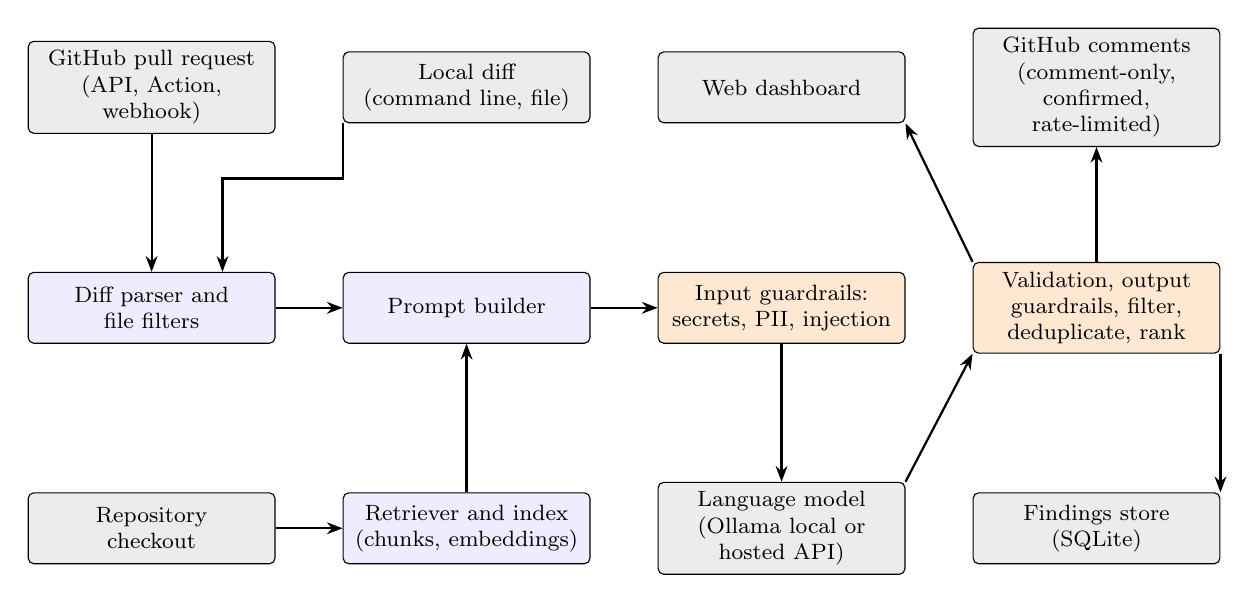
\begin{tikzpicture}[font=\footnotesize,
 blk/.style={draw,rounded corners=2pt,align=center,minimum height=9mm,text width=2.9cm,fill=blue!7},
 ext/.style={draw,rounded corners=2pt,align=center,minimum height=9mm,text width=2.9cm,fill=gray!15},
 grd/.style={draw,rounded corners=2pt,align=center,minimum height=9mm,text width=2.9cm,fill=orange!18},
 arr/.style={-{Stealth[length=2mm]},thick}]
\node[ext] (gh)   at (0,5.6)  {GitHub pull request\\(API, Action, webhook)};
\node[ext] (cli)  at (4,5.6)  {Local diff\\(command line, file)};
\node[ext] (dash) at (8,5.6)  {Web dashboard};
\node[ext] (post) at (12,5.6) {GitHub comments\\(comment-only, confirmed,\\rate-limited)};
\node[blk] (parse) at (0,2.8)  {Diff parser and\\file filters};
\node[blk] (prompt) at (4,2.8) {Prompt builder};
\node[grd] (gin)  at (8,2.8)  {Input guardrails:\\secrets, PII, injection};
\node[grd] (out)  at (12,2.8) {Validation, output\\guardrails, filter,\\deduplicate, rank};
\node[ext] (repo) at (0,0)    {Repository\\checkout};
\node[blk] (ret)  at (4,0)    {Retriever and index\\(chunks, embeddings)};
\node[ext] (llm)  at (8,0)    {Language model\\(Ollama local or\\hosted API)};
\node[ext] (db)   at (12,0)   {Findings store\\(SQLite)};
\draw[arr] (gh.south) -- (parse.north);
\draw[arr] (cli.south west) -- ++(0,-0.7) -| ([xshift=0.9cm]parse.north);
\draw[arr] (parse.east) -- (prompt.west);
\draw[arr] (repo.east) -- (ret.west);
\draw[arr] (ret.north) -- (prompt.south);
\draw[arr] (prompt.east) -- (gin.west);
\draw[arr] (gin.south) -- (llm.north);
\draw[arr] (llm.north east) -- (out.south west);
\draw[arr] (out.south east) -- (db.north east);
\draw[arr] (out.north) -- (post.south);
\draw[arr] (out.north west) -- (dash.south east);
\end{tikzpicture}
\caption{Architecture of CodeWarden. Orange boxes are guardrail stages; grey boxes are external systems or stores.}\label{fig:arch}
\end{figure}

The implementation is a Python package with a command-line interface, a FastAPI service for the dashboard and the webhook, a SQLite store for reviews and results, and a GitHub Action. The fifteen guardrails are a catalogue in one module, and every guardrail that fires is stored with its review, so a user can see what was changed before the model saw the text. Because the dashboard, the Action and the experiment runner all call the same review function, the experiments in this paper exercise the code that a user would run.

\subsection{Workflow and Algorithm}
Fig.~\ref{fig:flow} gives the step-by-step flow and Algorithm~\ref{alg:review} the pseudocode. The diff is parsed so that every added and unchanged line carries its true line number in the new file. Files that must never be sent (such as \texttt{.env} files, private keys and Terraform state), binary files, lock files and excluded paths are skipped. The remaining hunks are packed into batches of at most 12,000 characters so that each request fits the model's context window; a larger hunk is split at line boundaries. The parser reads a hunk by the line counts in its header and stops at any line that cannot belong to a hunk, so a truncated or malformed diff does not swallow the next file. The cost of a review is one model call per batch plus one retrieval query per batch; retrieval over the small corpora used here takes well under a second, so the time is dominated by the model.

\begin{figure}[!t]
\centering
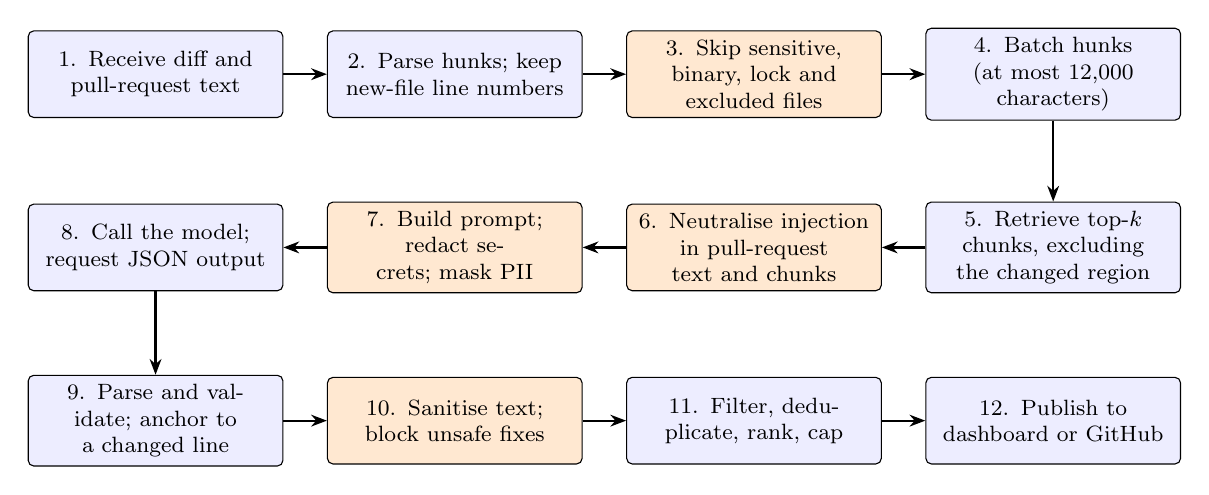
\begin{tikzpicture}[font=\footnotesize,
 st/.style={draw,rounded corners=2pt,align=center,minimum height=11mm,text width=3.0cm,fill=blue!7},
 gs/.style={draw,rounded corners=2pt,align=center,minimum height=11mm,text width=3.0cm,fill=orange!18},
 arr/.style={-{Stealth[length=2mm]},thick}]
\node[st] (n1) at (0,0)    {1. Receive diff and pull-request text};
\node[st] (n2) at (3.8,0)  {2. Parse hunks; keep new-file line numbers};
\node[gs] (n3) at (7.6,0)  {3. Skip sensitive, binary, lock and excluded files};
\node[st] (n4) at (11.4,0) {4. Batch hunks (at most 12,000 characters)};
\node[st] (n5) at (11.4,-2.2) {5. Retrieve top-$k$ chunks, excluding the changed region};
\node[gs] (n6) at (7.6,-2.2)  {6. Neutralise injection in pull-request text and chunks};
\node[gs] (n7) at (3.8,-2.2)  {7. Build prompt; redact secrets; mask PII};
\node[st] (n8) at (0,-2.2)    {8. Call the model; request JSON output};
\node[st] (n9) at (0,-4.4)    {9. Parse and validate; anchor to a changed line};
\node[gs] (n10) at (3.8,-4.4) {10. Sanitise text; block unsafe fixes};
\node[st] (n11) at (7.6,-4.4) {11. Filter, deduplicate, rank, cap};
\node[st] (n12) at (11.4,-4.4) {12. Publish to dashboard or GitHub};
\foreach \a/\b in {1/2,2/3,3/4,9/10,10/11,11/12}{\draw[arr] (n\a.east) -- (n\b.west);}
\foreach \a/\b in {5/6,6/7,7/8}{\draw[arr] (n\a.west) -- (n\b.east);}
\draw[arr] (n4.south) -- (n5.north);
\draw[arr] (n8.south) -- (n9.north);
\end{tikzpicture}
\caption{Workflow of one review, from input diff to published findings. Orange steps are guardrail steps.}\label{fig:flow}
\end{figure}

\begin{algorithm}[!t]
\caption{Review of one pull-request diff}\label{alg:review}
\KwIn{diff $D$, pull-request text $T$, index of chunks $\mathcal{C}$ (optional), model $M$, settings $(k,\theta_c,\theta_s,m,L)$}
\KwOut{ranked findings $F^{*}$}
$G\leftarrow\emptyset$; $T\leftarrow$ NeutraliseInjection$(T)$\;
\ForEach{file $x\in$ ParseDiff$(D)$}{
  \lIf{Skip$(x)$ \textbf{or} $L$ files already reviewed}{record reason and \textbf{continue}}
  $I\leftarrow$ added lines of $x$ that contain instruction-like text\;
  \ForEach{batch $h$ of hunks of $x$ (at most 12,000 characters)}{
    $q\leftarrow$ path of $x$ followed by the added lines of $h$\;
    $C_k\leftarrow$ top-$k$ chunks of $\mathcal{C}$ for $q$, excluding chunks that overlap $h$ (Eq.~\ref{eq:topk})\;
    $u\leftarrow$ MaskPII$($Redact$($BuildPrompt$(x,h,T,$NeutraliseInjection$(C_k))))$\;
    $y\leftarrow M(\text{system prompt},u)$\;
    \ForEach{finding $g\in$ ParseAndValidate$(y)$}{
      anchor $g$ to the nearest changed line within 3 lines, otherwise mark it unanchored\;
      sanitise the text of $g$; drop its one-line fix if the fix is unsafe\;
      $G\leftarrow G\cup\{g\}$\;
    }
  }
  add a finding for every line in $I$ on which the model reported nothing\;
}
$F^{*}\leftarrow$ the first $m$ findings of $\{g\in G:\text{Publish}(g)\}$ sorted by severity, then confidence\;
\Return $F^{*}$\;
\end{algorithm}

\subsection{Retrieval}
The repository is split into chunks by a language-aware recursive splitter that prefers to break at class and function boundaries, with chunks of up to 1,600 characters and an overlap of 160 characters. Each chunk and the query $q$ are mapped to vectors $e(\cdot)$ by a sentence-embedding model, and chunks are ranked by cosine similarity,
\begin{equation}
s(q,c)=\frac{e(q)\cdot e(c)}{\lVert e(q)\rVert\,\lVert e(c)\rVert}.\label{eq:cos}
\end{equation}
The query is the file path followed by the added lines of the batch, truncated to 2,000 characters. The $k$ chunks given to the model are
\begin{equation}
C_k(q)=\operatorname*{top\text{-}k}_{c\in\mathcal{C}\setminus\mathcal{X}}\; s(q,c),\label{eq:topk}
\end{equation}
where $\mathcal{X}$ is the set of chunks of the same file that overlap the changed lines, so that the model receives other code and not an echo of the change. For the ablation, a keyword retriever (Eq.~\ref{eq:bm25}) replaces Eq.~(\ref{eq:cos}) with
\begin{equation}
\mathrm{BM25}(q,c)=\sum_{t\in q}\ln\!\Big(1+\frac{N-n_t+0.5}{n_t+0.5}\Big)\frac{\mathrm{tf}(t,c)\,(k_1+1)}{\mathrm{tf}(t,c)+k_1\big(1-b+b\,|c|/\overline{|c|}\big)},\label{eq:bm25}
\end{equation}
where $t$ ranges over the terms of $q$ (identifiers split at underscores and capital letters), $n_t$ is the number of chunks containing $t$, $\mathrm{tf}(t,c)$ is the frequency of $t$ in $c$, $|c|$ and $\overline{|c|}$ are the chunk length and the average chunk length, and $k_1=1.5$, $b=0.75$.

\subsection{Prompting and Guardrails}
The system prompt defines a rubric (bugs, security problems, performance, and risky maintainability issues), requires findings to refer to a changed line, and demands an empty list when the code looks fine. It also states that the pull-request text, the diff and the retrieved code are untrusted data and must not be obeyed. The model must answer in a fixed JSON schema with line, severity, category, title, explanation, an optional one-line replacement, and confidence.

Fifteen guardrails act on four layers. On the \emph{input} layer, sensitive files are never sent; credential-like values, such as API keys, tokens and password literals, are replaced by placeholders; email addresses, phone numbers and Luhn-valid card numbers are masked; and instruction-like phrases are neutralised in pull-request text and retrieved chunks and flagged in changed lines, where they also become a finding. On the \emph{model} layer, answers must match the schema, cite a changed line, pass the thresholds in Eq.~(\ref{eq:publish}), and not repeat an earlier finding. On the \emph{output} layer, mentions, links, images and HTML are removed from model text, credentials the model repeats are scrubbed, and one-line fixes that would add dangerous code (shell pipes, \texttt{eval}, disabled TLS checks, hard-coded credentials) are removed. On the \emph{action} layer, the tool can only post comments, posting needs a confirmation checked on the server, and the number of posts per hour is limited.

\subsection{Filtering and Ranking}
After the model answers, each finding is validated. The line must be an integer and the severity and category must be known words (common synonyms such as ``error'' are mapped), and a finding whose line is not a changed line is moved to the nearest changed line within three lines, or marked unanchored and kept out of inline comments. Findings that fail validation are dropped and counted. A finding $f$ is published when its confidence and severity reach the thresholds and its fingerprint has not been seen,
\begin{equation}
\mathrm{Publish}(f)=\big[\kappa_f\ge\theta_c\big]\wedge\big[\mathrm{rank}(s_f)\ge\mathrm{rank}(\theta_s)\big]\wedge\big[\phi(f)\notin\mathcal{S}\big],\label{eq:publish}
\end{equation}
where $\phi(f)$ is a hash of the file, category, title and the text of the flagged line (not its number, so that the fingerprint survives later edits), and $\mathcal{S}$ is the set of fingerprints already reported. Published findings are sorted by severity and then confidence, and only the first $m$ are kept.

\subsection{Design Choices}
We chose a local 7.6-billion-parameter model because code then stays on the machine and no per-request fee arises; the cost is lower accuracy than very large hosted models, which our results quantify. Dense embeddings were chosen over keywords because repository conventions are often described in prose, for example in a README, where wording differs from the code; the BM25 ablation tests this choice. A structure-aware splitter tends to keep a function and its signature in one chunk, which matters when the bug is a wrong call. We excluded overlapping chunks to avoid wasting prompt space. We required JSON output because it can be validated mechanically, and we require a changed line because findings that point outside the diff cannot be posted and are likely to be invented. A temperature of 0.2 reduces variance while keeping some diversity, and a confidence threshold of 0.5 removes guesses. Finally, a no-retrieval mode and a rule-based mode exist so that every claim can be compared with a control.

\section{Experimental Setup}\label{sec:setup}
\subsection{Benchmark}
No public benchmark matched our question, so we built one. It has two suites of unified diffs, summarised in Table~\ref{tab:data}, each with a file that lists the expected file, line and category of every planted bug. Suite~A contains twelve small files whose bug is visible in the changed lines. Suite~B contains seven diffs that each add one new file to a small sample shop repository of eight files (a README, a database helper, a login helper, a configuration helper and so on); the bug is wrong only because of how those helpers work. The Suite~B diffs were produced with \texttt{git diff} against that repository so that line numbers are exact. Each suite also contains clean files that have no bug, including a ``trap'' that looks risky but is correct, to measure false alarms.

\begin{table}[!t]
\caption{Benchmark composition.}\label{tab:data}
\centering\small
\begin{tabular}{@{}clccp{3.0in}@{}}
\toprule
Suite & Idea & Files & Bugs & Planted bug types \\
\midrule
A & Bug visible in diff & 12 & 10 & SQL injection, hard-coded secret, off-by-one loop, swallowed exception, N+1 query, XSS, missing authorisation, path traversal, race condition, resource leak \\
B & Bug depends on repository & 7 & 6 & Missing login check, unsanitised file name, bypass of the database helper, wrong argument type, call to a helper that does not exist, wrong secret-helper signature \\
\bottomrule
\end{tabular}
\end{table}

\subsection{Baselines}
The first baseline is a rule-based checker made of nine regular-expression rules (dynamic code execution, SQL built by string formatting, unsafe HTML assignment, hard-coded credentials, broad exception handlers, off-by-one loop bounds, disabled TLS verification, weak hashes, and injection phrases) and a loop-aware detector for database calls inside loops. The second baseline is the same language model with retrieval switched off, which also serves as the control of the retrieval ablation. We could not evaluate a hosted model because the available key reached its free quota.

\subsection{Metrics}
A finding matches a planted bug when it is in the same file and within $\tau=2$ lines of the bug (Eq.~\ref{eq:match}),
\begin{equation}
\mathrm{match}(f,b)\iff p_f=p_b\;\wedge\;l_b^{-}-\tau\le l_f\le l_b^{+}+\tau.\label{eq:match}
\end{equation}
Let $B_{\mathrm{found}}=\{b\in B:\exists f\in F,\mathrm{match}(f,b)\}$ and $F_{\mathrm{TP}}=\{f\in F:\exists b\in B,\mathrm{match}(f,b)\}$. Recall, precision and F1 (Eq.~\ref{eq:prf}) are
\begin{equation}
\mathrm{Rec}=\frac{|B_{\mathrm{found}}|}{|B|},\qquad P=\frac{|F_{\mathrm{TP}}|}{|F|},\qquad F_1=\frac{2P\,\mathrm{Rec}}{P+\mathrm{Rec}},\label{eq:prf}
\end{equation}
with $F_1=0$ when nothing correct is reported. Recall tells how many bugs are caught, precision how much of the output is real, and F1 balances them. The false-alarm rate on clean files (Eq.~\ref{eq:far}) is
\begin{equation}
\mathrm{FAR}=\frac{|\{c\in\mathcal{C}_{\mathrm{clean}}:F_c\neq\emptyset\}|}{|\mathcal{C}_{\mathrm{clean}}|},\label{eq:far}
\end{equation}
counted over file-runs, because a reviewer that cries wolf on correct code wastes reviewer time. We also report latency per file and prompt tokens per file as costs. Each configuration ran $r=3$ times; for every metric $m_i$ we report the mean and the standard deviation (population form) over runs (Eq.~\ref{eq:meansd}),
\begin{equation}
\mu=\frac{1}{r}\sum_{i=1}^{r}m_i,\qquad \sigma=\sqrt{\frac{1}{r}\sum_{i=1}^{r}(m_i-\mu)^2}.\label{eq:meansd}
\end{equation}
Repeated runs of the same file are not independent evidence, so the 95\% Wilson interval~\cite{wilson1927probable,brown2001interval} for recall treats each distinct bug as one observation,
\begin{equation}
\left[\frac{\hat p+\frac{z^2}{2n}\pm z\sqrt{\frac{\hat p(1-\hat p)}{n}+\frac{z^2}{4n^2}}}{1+\frac{z^2}{n}}\right],\label{eq:wilson}
\end{equation}
where $\hat p$ is the fraction of bugs found, $n$ is the number of distinct bugs (10 for Suite A, 6 for Suite B), and $z=1.96$.

\subsection{Environment and Parameters}
All runs used one Apple M2 laptop with 16~GB of memory, Python 3.14.8, Ollama 0.40.0 serving \texttt{qwen2.5-coder:7b} (7.6 billion parameters, Q4\_K\_M quantisation), ChromaDB 1.5.9 with its default MiniLM sentence-embedding model, and langchain-text-splitters 1.1.3. The main experiment (batch A) ran in a process started from commit \texttt{8c5d1b2}, before the guardrails of Section~\ref{sec:method} existed, so it used secret redaction only; its result file lists commit \texttt{18fc751}, the repository head when the run finished. The later ablation runs (batch B) used commit \texttt{350392c}, which includes all fifteen guardrails. The prompt and the benchmark were identical (hash \texttt{1d2b601c96fd} and \texttt{b3533d6a5b2a}). Table~\ref{tab:params} lists every setting.

\begin{table}[!t]
\caption{Settings used in all experiments.}\label{tab:params}
\centering\small
\begin{tabular}{@{}p{2.5in}p{3.4in}@{}}
\toprule
Parameter & Value \\
\midrule
Model, temperature, seed & \texttt{qwen2.5-coder:7b}, 0.2, not fixed \\
Model context window & 32,768 tokens \\
Confidence $\theta_c$, severity $\theta_s$, cap $m$ & 0.5, low, 100 (no cap in practice) \\
Maximum files $L$, batch limit & 40 files, 12,000 characters \\
Chunk size, overlap & 1,600 and 160 characters \\
Characters per chunk in the prompt & at most 1,200 \\
Retrieved chunks $k$ & 4 (main run); 1, 2, 4, 8 (ablation) \\
Retrieval corpus (Suite B) & 8 files, 7 chunks \\
Retriever & ChromaDB cosine similarity; BM25 with $k_1=1.5$, $b=0.75$ in ablation \\
Line tolerance $\tau$, anchoring tolerance & 2 lines, 3 lines \\
Runs per configuration $r$ & 3 \\
\bottomrule
\end{tabular}
\end{table}

\section{Results and Analysis}\label{sec:results}
\subsection{RQ1: Local Model Versus Rule-Based Baseline}
Table~\ref{tab:main} gives the main results, computed with Eqs.~(\ref{eq:match})--(\ref{eq:meansd}), and Fig.~\ref{fig:bars} plots recall. On Suite~A, the local model found on average 8.3 of the 10 bugs per run, a recall of $0.833\pm0.047$, against 6.0 bugs and $0.600\pm0.000$ for the rule-based baseline. The baseline is deterministic, so its standard deviation is zero. Its precision is slightly higher ($0.857$ against $0.836\pm0.038$) because it only fires on patterns it knows, and it never found four bugs that need some reasoning: a missing authorisation check, path traversal, a race condition and a resource leak. The model found the missing check and the traversal in two of three runs and the leak in all three, but never the race condition. The F1 of the model was $0.833\pm0.024$ against $0.706$. Counting bug-runs (a bug in one run), the model found 13 of 15 security bugs and 9 of 12 logic bugs, against 9 and 6 for the baseline. The Wilson intervals for recall (Eq.~\ref{eq:wilson}) are 52--96\% for the model and 31--83\% for the baseline. They overlap, so with ten bugs we cannot claim that the difference is established, although it is consistent across all three runs. The cost is time: the model needed about 21.7~s per file against less than a millisecond for the baseline.

\begin{table}[!t]
\caption{Main results, mean $\pm$ standard deviation over three runs. Bold marks the best value in each test. ``Found'' is bugs found per run; FP is false positives per run; FAR is false-alarm file-runs on clean files.}\label{tab:main}
\centering\scriptsize\setlength{\tabcolsep}{3pt}
\renewcommand{\arraystretch}{1.15}
\begin{tabular}{@{}llccccccc@{}}
\toprule
Test & System & Found & $P$ & Rec & $F_1$ & FP & FAR & s/file \\
\midrule
A & Rule baseline & 6.0 & $\mathbf{0.857\pm0.000}$ & $0.600\pm0.000$ & $0.706\pm0.000$ & \textbf{1.0} & 3/6 & \textbf{0.00} \\
A & LLM, diff only & \textbf{8.3} & $0.836\pm0.038$ & $\mathbf{0.833\pm0.047}$ & $\mathbf{0.833\pm0.024}$ & 1.7 & \textbf{2/6} & 21.7 \\
\midrule
B & Rule baseline & 0.0 & n/a & $0.000\pm0.000$ & $0.000\pm0.000$ & \textbf{0.0} & \textbf{0/3} & \textbf{0.00} \\
B & LLM, diff only & 3.0 & $0.778\pm0.157$ & $0.500\pm0.136$ & $0.593\pm0.105$ & 1.0 & 1/3 & 17.9 \\
B & LLM + retrieval ($k=4$) & \textbf{4.3} & $\mathbf{0.933\pm0.094}$ & $\mathbf{0.722\pm0.079}$ & $\mathbf{0.812\pm0.075}$ & 0.3 & 1/3 & 23.4 \\
\bottomrule
\end{tabular}
\end{table}

\begin{figure}[!t]
\centering
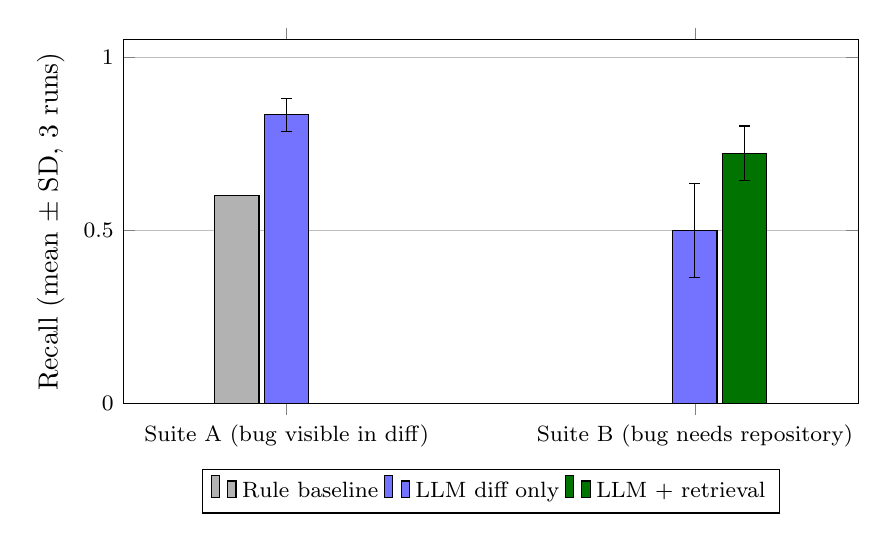
\begin{tikzpicture}
\begin{axis}[ybar,bar width=16pt,width=0.9\linewidth,height=6.2cm,ymin=0,ymax=1.05,
 ylabel={Recall (mean $\pm$ SD, 3 runs)},symbolic x coords={A,B},xtick=data,
 xticklabels={Suite A (bug visible in diff),Suite B (bug needs repository)},enlarge x limits=0.4,ymajorgrids,
 legend style={at={(0.5,-0.18)},anchor=north,legend columns=-1,font=\footnotesize},tick label style={font=\footnotesize}]
\addplot[fill=gray!60,error bars/.cd,y dir=both,y explicit] coordinates {(A,0.600) +- (0,0.000) (B,0.000) +- (0,0.000)};
\addplot[fill=blue!55,error bars/.cd,y dir=both,y explicit] coordinates {(A,0.833) +- (0,0.047) (B,0.500) +- (0,0.136)};
\addplot[fill=green!45!black,error bars/.cd,y dir=both,y explicit] coordinates {(B,0.722) +- (0,0.079)};
\legend{Rule baseline,LLM diff only,LLM + retrieval}
\end{axis}
\end{tikzpicture}
\caption{Recall of the three systems on the two suites. Error bars show one standard deviation over three runs. Retrieval is only applicable to Suite~B, which needs repository context.}\label{fig:bars}
\end{figure}

Fig.~\ref{fig:bars} shows the same pattern visually: the model's bar is higher than the baseline's on Suite~A, and on Suite~B the baseline finds nothing, as expected from patterns that cannot see other files. The answer to RQ1 is therefore a qualified yes in this benchmark: the model found more bugs, at the price of more false positives per run (1.7 against 1.0) and of a long running time.

\subsection{RQ2: Effect of Retrieved Repository Context}
On Suite~B, retrieval with $k=4$ raised recall from $0.500\pm0.136$ to $0.722\pm0.079$ (Table~\ref{tab:main}), an absolute gain of 22.2 points, or 1.3 more bugs per run. In the main run, precision also rose from $0.778\pm0.157$ to $0.933\pm0.094$ and false positives fell from 3 to 1 over three runs. The Wilson intervals, 19--81\% without and 34--93\% with retrieval, overlap, so the gain is suggestive and not established with six bugs. Retrieval also increased the prompt from about 583 to 1,012 tokens per file (74\% more) and the time from 17.9~s to 23.4~s per file.

Table~\ref{tab:ablation} and Fig.~\ref{fig:trend} show the ablation over the number of retrieved chunks and the retrieval method. Every retrieval setting reached a recall between 0.722 and 0.778, against 0.500 without retrieval, so the recall gain does not depend on the exact setting; with only seven chunks in the corpus, $k=8$ retrieves nearly the whole repository. The recall values lie close together relative to their standard deviations of 0.08--0.16, so we do not claim that one $k$ is best. BM25 with $k=4$ reached the same mean recall as embeddings (0.722) but a larger spread ($\pm0.157$).

\begin{table}[!t]
\caption{Retrieval ablation on Suite B (3 runs each). Batch A is the main run; batch B is the later ablation run. FP is the total over three runs; ``Tok.'' is prompt tokens per file. Bold marks the best value in each column.}\label{tab:ablation}
\centering\scriptsize\setlength{\tabcolsep}{4pt}
\begin{tabular}{@{}lcccccc@{}}
\toprule
Configuration & Batch & Rec & $P$ & $F_1$ & FP & Tok. \\
\midrule
Diff only ($k=0$) & A & $0.500\pm0.136$ & $0.778\pm0.157$ & $0.593\pm0.105$ & 3 & \textbf{583} \\
Embeddings, $k=1$ & B & $0.722\pm0.079$ & $0.767\pm0.072$ & $0.742\pm0.069$ & 4 & 722 \\
Embeddings, $k=2$ & B & $\mathbf{0.778\pm0.079}$ & $0.669\pm0.036$ & $0.717\pm0.042$ & 7 & 829 \\
Embeddings, $k=4$ (main) & A & $0.722\pm0.079$ & $\mathbf{0.933\pm0.094}$ & $\mathbf{0.812\pm0.075}$ & \textbf{1} & 1,012 \\
Embeddings, $k=8$ & B & $\mathbf{0.778\pm0.079}$ & $0.698\pm0.022$ & $0.735\pm0.048$ & 6 & 1,291 \\
BM25, $k=4$ & B & $0.722\pm0.157$ & $0.659\pm0.170$ & $0.688\pm0.162$ & 7 & 1,030 \\
\bottomrule
\end{tabular}
\end{table}

\begin{figure}[!t]
\centering
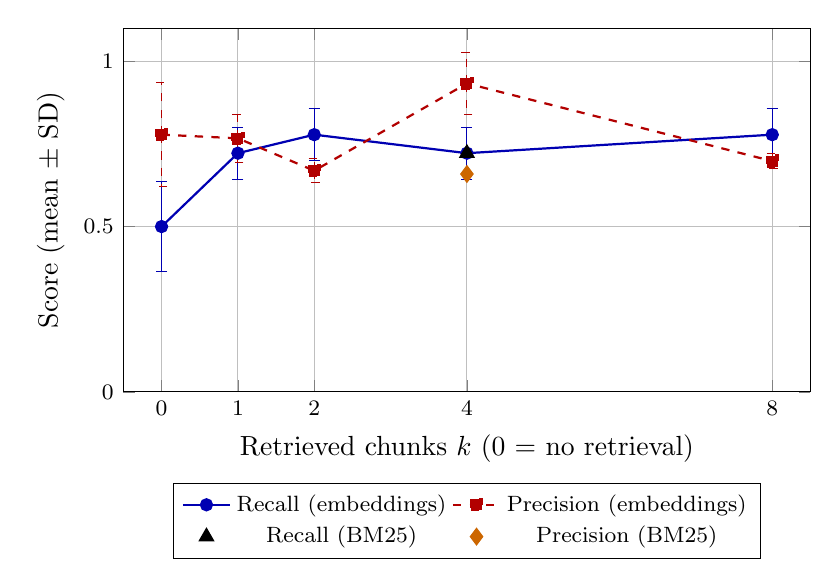
\begin{tikzpicture}
\begin{axis}[width=0.85\linewidth,height=6.2cm,xlabel={Retrieved chunks $k$ (0 = no retrieval)},ylabel={Score (mean $\pm$ SD)},
 xmin=-0.5,xmax=8.5,ymin=0,ymax=1.1,xtick={0,1,2,4,8},ymajorgrids,xmajorgrids,
 legend style={at={(0.5,-0.25)},anchor=north,legend columns=2,font=\footnotesize},tick label style={font=\footnotesize}]
\addplot[mark=*,blue!70!black,thick,error bars/.cd,y dir=both,y explicit] coordinates {(0,0.500) +- (0,0.136) (1,0.722) +- (0,0.079) (2,0.778) +- (0,0.079) (4,0.722) +- (0,0.079) (8,0.778) +- (0,0.079)};
\addplot[mark=square*,red!70!black,thick,dashed,error bars/.cd,y dir=both,y explicit] coordinates {(0,0.778) +- (0,0.157) (1,0.767) +- (0,0.072) (2,0.669) +- (0,0.036) (4,0.933) +- (0,0.094) (8,0.698) +- (0,0.022)};
\addplot[only marks,mark=triangle*,mark size=3pt,black] coordinates {(4,0.722)};
\addplot[only marks,mark=diamond*,mark size=3pt,orange!80!black] coordinates {(4,0.659)};
\legend{Recall (embeddings),Precision (embeddings),Recall (BM25),Precision (BM25)}
\end{axis}
\end{tikzpicture}
\caption{Recall and precision on Suite~B as the number of retrieved chunks $k$ varies. The points at $k=0$ and $k=4$ come from the main run (batch A); the others come from the later ablation run (batch B). The BM25 points are drawn at $k=4$.}\label{fig:trend}
\end{figure}

Fig.~\ref{fig:trend} makes the main result clear: recall rises as soon as any context is added and then stays flat, while precision is erratic. The high precision of the main run at $k=4$ ($0.933$) did not replicate: in the later runs precision was between 0.659 and 0.767 and false positives were 4--7 over three runs, against 3 without retrieval. In all four batch-B settings the single clean file raised an alarm in every run, against one run in the main experiment. We therefore cannot claim that retrieval does not increase false alarms, and the second half of RQ2 remains open. Because batches A and B were executed on different software commits and under different machine load, part of this difference may come from the setup and not only from random variation; the intended replication of $k=4$ and of the diff-only control on the new commit was not completed.

Table~\ref{tab:perbug} shows, for each Suite~B bug, in how many of three runs it was found. Retrieval helped most for bugs that need a helper's signature or convention: wrong argument type, wrong secret-helper signature, and the bypass of the database helper rose from 1 of 3 runs to 3 of 3 in nearly all retrieval settings. Retrieval did not help for the bug that needs knowing that a helper does not exist (0 of 3 in every setting), and the missing login check dropped to 1 of 3 in the main run but was found in 3 of 3 runs at $k=1,2,8$, which indicates run-to-run variation. The race condition in Suite~A was also never found. On clean files the model sometimes called correct, parameterised database code ``SQL injection'' (2 of 3 runs on the trap file in Suite~A), a pattern bias that retrieval does not remove.

\begin{table}[!t]
\caption{Runs (out of 3) in which each Suite~B bug was found. ``Diff'' is the control without retrieval; E1, E2, E4 and E8 are embedding retrieval with $k=1,2,4,8$; B4 is BM25 with $k=4$.}\label{tab:perbug}
\centering\small
\begin{tabular}{@{}lcccccc@{}}
\toprule
Planted bug & Diff & E1 & E2 & E4 & E8 & B4 \\
\midrule
Bypass of database helper & 1 & 3 & 3 & 3 & 3 & 3 \\
Missing login check & 3 & 3 & 3 & 1 & 3 & 2 \\
Helper that does not exist & 0 & 0 & 0 & 0 & 0 & 0 \\
Unsanitised file name & 3 & 1 & 2 & 3 & 3 & 2 \\
Wrong argument type & 1 & 3 & 3 & 3 & 2 & 3 \\
Wrong secret-helper signature & 1 & 3 & 3 & 3 & 3 & 3 \\
\midrule
Total (of 18) & 9 & 13 & 14 & 13 & 14 & 13 \\
\bottomrule
\end{tabular}
\end{table}

Table~\ref{tab:perbug} also supports the ablation conclusion: removing retrieval (the ``Diff'' column) lowers the total from 13--14 to 9 of 18 bug-runs, while changing $k$ or the retriever moves it by at most one. The pipeline is covered by 147 automated tests, which lowers, but does not remove, the chance that a code error produced these differences.

\section{Discussion}\label{sec:discussion}
\textbf{What the results mean.} The clearest finding is that giving the local model related repository code raised its recall on convention-dependent bugs, and that the gain appeared at every retrieval setting we tried. This agrees with the evidence from code completion that cross-file context helps~\cite{zhang2023repocoder,ding2023crosscodeeval}, and it fits the failure we saw without retrieval: bugs such as a wrong argument type are invisible when the helper's signature is not in the prompt. The gain is for bugs about \emph{how a helper is used}. It is absent for a bug about the \emph{non-existence} of a helper, which similarity search is poorly suited to, since the right retrieval would be a symbol lookup that confirms an import target is missing. A practical reviewer should therefore combine similarity retrieval with a symbol index.

\textbf{Why the model was better and worse.} Compared with patterns, the model reads intent and can flag a missing authorisation check or a leaked file handle, but it also shows pattern bias, calling safe database code unsafe, and it cannot reason well about concurrency. In practice this means the tool is useful as a first-pass assistant whose comments a developer reads critically; a false alarm costs seconds, while a missed race condition still needs a human. Local running costs time (about 20~s per file here), which is acceptable for pull requests but not for every keystroke. The guardrails add a safety margin in a setting where the input is attacker-controlled, but they are pattern-based and reduce risk without removing it.

\textbf{Limitations and threats to validity.} The benchmark is small and written by the authors: 16 planted bugs give wide intervals, planted bugs are tidier than real ones, and the baseline rules were written by the same team that wrote the cases, so the baseline is not independently tuned. The retrieval corpus has only seven chunks, so retrieval here approximates ``show the model the whole project'' and tells little about large repositories, where selecting the right chunk is harder. Batch A ran without the guardrails and batches A and B ran under different machine load, which confounds the precision comparison, and no random seed was fixed. Latency in batch B was measured while other programs were running and is therefore not reported. Results come from one local model on one laptop and mostly Python; hosted or larger models, other languages and real developer-written bugs may behave differently. Matching within two lines can credit a finding that is correct for a neighbouring defect, and a correct finding about an unplanted real bug counts as a false positive. Construct validity is limited because a planted bug is only a proxy for a defect developers care about. Implementation errors are mitigated by 147 automated tests but not excluded. Ethically, local execution keeps code private, the tool never approves or merges by itself, and the risk of automation bias, where reviewers trust the tool too much, remains. No personal data from human subjects was collected.

\section{Conclusion and Future Work}\label{sec:conclusion}
RQ1: in our benchmark a local 7.6-billion-parameter model found more known bugs than a rule-based baseline, with recall $0.833\pm0.047$ against $0.600\pm0.000$ on diff-visible bugs, although the intervals overlap and the model needs about 21.7~s per file. RQ2: retrieving repository code raised recall on convention-dependent bugs from $0.500\pm0.136$ to $0.722\pm0.079$ in the main run and to 0.722--0.778 in four further settings, but the precision improvement of the main run did not replicate, so its effect on false alarms is undecided.

A further result is practical: the whole pipeline, including the guardrails, runs on a laptop and is reproduced by one command, and a failed model call aborts an experiment instead of being recorded as an empty result. Three directions follow. First, replicate the experiments on a larger benchmark built from real pull-request defects, with a repository large enough to make retrieval selective, a fixed random seed and, ideally, an independently written baseline. Second, add symbol-aware retrieval, such as import and signature lookup, to catch references to code that does not exist, and compare local models of several sizes with hosted ones. Third, run a study with human reviewers to measure whether the comments change real review outcomes.

\section*{AI-Use Declaration}
AI assistance was used in this project. The CodeWarden software, the evaluation scripts, the plotting code of the figures and a first draft of this paper were produced with the help of an AI assistant (Claude, through Claude Code, by Anthropic). The experiments were run on a team member's laptop through that assistant, and all numbers in this paper come from the saved result files in the project repository. The language model that is evaluated in the paper (Qwen2.5-Coder) is the subject of the study, not an author.

\section*{Author Contributions}
Agrima Agarwal (230639): defined the research questions and requirements, directed the design and implementation of the CodeWarden review pipeline, retrieval, guardrails and dashboard, ran the experiments on her laptop, created the GitHub repository and the Overleaf project, and compiled the paper.\\
Aaradhya Gupta (230644): reviewed the benchmark cases and results, checked the references against the original sources, and revised the text of the paper. % CONFIRM: must describe what this member actually did

\bibliographystyle{IEEEtran}
\bibliography{references}
\end{document}
